% SkripsiBench paper — IEEE conference format
% Build: paper-agent compile paper_bench/main.tex   (tables in generated/ come from paper_bench/make_tables.py)
\documentclass[conference]{IEEEtran}
\IEEEoverridecommandlockouts

\usepackage[utf8]{inputenc}
\usepackage[T1]{fontenc}
\usepackage{cite}
\usepackage{amsmath,amssymb,amsfonts}
\usepackage{graphicx}
\usepackage{booktabs}
\usepackage{array}
\usepackage{multirow}
\usepackage{xcolor}
\usepackage{url}
\usepackage[hidelinks]{hyperref}
\usepackage{microtype}

\graphicspath{{figures/}}

% \todo{} marks items that must be resolved before submission
\newcommand{\todo}[1]{\textcolor{red}{[TODO: #1]}}
\newcommand{\task}[1]{\texttt{#1}}
% generated tables: English (main.tex) or Indonesian captions (main_id.tex); numbers come from the run data
\newcommand{\langsuffix}{}
% generated by paper_bench/make_tables.py from experiments/bench/{summary,analysis,refs_audit}.json — do not edit
\newcommand{\NModels}{25}
\newcommand{\NApi}{15}
\newcommand{\NLocal}{10}
\newcommand{\NItems}{255}
\newcommand{\NApiCalls}{7{,}356}
\newcommand{\NBenchCalls}{3{,}852}
\newcommand{\NJudgeCalls}{3{,}480}
\newcommand{\NLocalCalls}{2{,}580}
\newcommand{\StudyUSD}{46.65}
\newcommand{\JudgeUSD}{24.50}
\newcommand{\AnswerUSD}{21.52}
\newcommand{\ProbeUSD}{0.63}
\newcommand{\TokensInM}{3.4}
\newcommand{\TokensOutM}{2.3}
\newcommand{\GpuHours}{6.1}
\newcommand{\GpuUSD}{6.70}
\newcommand{\TopName}{kimi-k3}
\newcommand{\TopScore}{0.941}
\newcommand{\SecondName}{gpt-5.4}
\newcommand{\ThirdName}{gpt-6.1-sol}
\newcommand{\FourthName}{claude-sonnet-5.5}
\newcommand{\FourthScore}{0.913}
\newcommand{\SecondScore}{0.935}
\newcommand{\ThirdScore}{0.931}
\newcommand{\DiffB}{0.006}
\newcommand{\DiffBLo}{$-$0.014}
\newcommand{\DiffBHi}{0.027}
\newcommand{\DiffC}{0.010}
\newcommand{\DiffCLo}{$-$0.010}
\newcommand{\DiffCHi}{0.028}
\newcommand{\DiffD}{0.028}
\newcommand{\DiffDLo}{0.006}
\newcommand{\DiffDHi}{0.050}
\newcommand{\NoSigN}{2}
\newcommand{\JudgeAutoRho}{0.994}
\newcommand{\JudgeOnlyRho}{0.996}
\newcommand{\JudgeAutoShift}{3}
\newcommand{\JudgeOnlyShift}{2}
\newcommand{\PubRho}{0.999}
\newcommand{\PubMaxShift}{1}
\newcommand{\TopFourMinP}{0.32}
\newcommand{\PTopA}{70}
\newcommand{\PTopB}{25}
\newcommand{\PTopC}{5}
\newcommand{\TopUSD}{3.12}
\newcommand{\SecondUSD}{0.86}
\newcommand{\ThirdUSD}{0.46}
\newcommand{\FourthUSD}{0.78}
\newcommand{\TopMedS}{34.5}
\newcommand{\ThirdMedS}{8.3}
\newcommand{\CheapName}{gpt-6-luna}
\newcommand{\CheapUSD}{0.030}
\newcommand{\CheapScore}{0.901}
\newcommand{\CheapCloseName}{gpt-6-luna}
\newcommand{\CheapCloseUSD}{0.030}
\newcommand{\CostRatio}{104}
\newcommand{\CheapGap}{0.04}
\newcommand{\ParetoN}{5}
\newcommand{\ParetoNames}{kimi-k3, gpt-5.4, gpt-6.1-sol, gemini-3.7-flash, gpt-6-luna}
\newcommand{\MethCeil}{15}
\newcommand{\LangCeil}{14}
\newcommand{\MethApiMin}{0.98}
\newcommand{\LangApiMin}{0.92}
\newcommand{\RefApiMin}{0.23}
\newcommand{\RefApiMax}{0.94}
\newcommand{\RefApiSD}{0.18}
\newcommand{\StructApiMin}{0.57}
\newcommand{\StructApiMax}{0.79}
\newcommand{\LatexApiMin}{0.79}
\newcommand{\ExtApiMin}{0.85}
\newcommand{\ExtApiMax}{0.97}
\newcommand{\HalApiMin}{0}
\newcommand{\HalApiMax}{40}
\newcommand{\HalLocMin}{74}
\newcommand{\HalLocMax}{95}
\newcommand{\DoiApiMin}{25}
\newcommand{\DoiApiMax}{98}
\newcommand{\BestLocalName}{Qwen3.6 36B}
\newcommand{\BestLocalScore}{0.745}
\newcommand{\WorstApiName}{claude-haiku-4.5}
\newcommand{\WorstApiScore}{0.777}
\newcommand{\GapRef}{0.59}
\newcommand{\GapCode}{0.47}
\newcommand{\GapLang}{0.08}
\newcommand{\GapMeth}{0.24}
\newcommand{\SahLang}{0.891}
\newcommand{\GemmaFourLang}{0.925}
\newcommand{\SahCode}{0.11}
\newcommand{\SahOverall}{0.517}
\newcommand{\GemmaFourOverall}{0.668}
\newcommand{\LocUSDMin}{0.07}
\newcommand{\LocUSDMax}{0.69}
\newcommand{\LocKwhMin}{0.012}
\newcommand{\LocKwhMax}{0.111}
\newcommand{\LocPassOneMin}{0.03}
\newcommand{\LocPassOneMax}{0.87}
\newcommand{\LocPassOneMean}{0.46}
\newcommand{\LocRepairMean}{0.61}
\newcommand{\ApiPassOneMin}{0.83}
\newcommand{\ApiPerfectCode}{9}
\newcommand{\AlphaJudges}{0.86}
\newcommand{\NAllJudges}{480}
\newcommand{\NJudgedAnswers}{1{,}500}
\newcommand{\AlphaCritMin}{0.46}
\newcommand{\AlphaCritMax}{0.80}
\newcommand{\LeniencyRange}{0.07}
\newcommand{\RhoModelGrd}{0.82}
\newcommand{\RhoModelLng}{0.82}
\newcommand{\RhoAnsGrd}{0.69}
\newcommand{\RhoAnsLng}{0.53}
\newcommand{\SilverUnanimous}{77}
\newcommand{\SilverAnalysisNone}{6}
\newcommand{\Substitutions}{no}
\newcommand{\GenericApiMin}{6}
\newcommand{\GenericApiMax}{34}
\newcommand{\FixApiMin}{0.50}
\newcommand{\ForeignLocMax}{93}
\newcommand{\ForeignLocMin}{0}
\newcommand{\LocMethMax}{1.00}
\newcommand{\LocMethMin}{0.40}
\newcommand{\LocLangMin}{0.80}
\newcommand{\LocLangMax}{0.96}
\newcommand{\ForeignApiMax}{10}
\newcommand{\UnsupApiMax}{0.17}
\newcommand{\NPremium}{9}
\newcommand{\AuditApiNF}{130}
\newcommand{\AuditApiExact}{17}
\newcommand{\AuditApiTitle}{4}
\newcommand{\AuditApiNone}{79}
\newcommand{\AuditLocNF}{681}
\newcommand{\AuditLocExact}{3}
\newcommand{\AuditLocTitle}{11}
\newcommand{\AuditLocNone}{86}
\newcommand{\AuditUnchecked}{0}
\newcommand{\NoneApiMin}{0}
\newcommand{\NoneApiMax}{31}
\newcommand{\NoneLocMin}{61}
\newcommand{\NoneLocMax}{85}
\newcommand{\NoneApiNonzero}{12}
\newcommand{\NoneApiZero}{3}
\newcommand{\VerRho}{0.999}
\newcommand{\VerRefRho}{0.998}
\newcommand{\VerMaxShift}{1}
\newcommand{\VerRefMaxGain}{0.03}
\newcommand{\VerOverallMaxGain}{0.004}
\newcommand{\VerLeaderSame}{yes}
\newcommand{\ScoreClaudeHaikuFourFive}{0.777}
\newcommand{\AcadClaudeHaikuFourFive}{0.762}
\newcommand{\CodeClaudeHaikuFourFive}{0.823}
\newcommand{\UsdClaudeHaikuFourFive}{0.598}
\newcommand{\KwhClaudeHaikuFourFive}{--}
\newcommand{\FabrClaudeHaikuFourFive}{40}
\newcommand{\DoiClaudeHaikuFourFive}{25}
\newcommand{\RefsClaudeHaikuFourFive}{2.8}
\newcommand{\PassOneClaudeHaikuFourFive}{0.83}
\newcommand{\RepairClaudeHaikuFourFive}{0.97}
\newcommand{\FixClaudeHaikuFourFive}{0.50}
\newcommand{\MedSClaudeHaikuFourFive}{10.6}
\newcommand{\ForeignClaudeHaikuFourFive}{0}
\newcommand{\GenericClaudeHaikuFourFive}{23}
\newcommand{\NoneClaudeHaikuFourFive}{31}
\newcommand{\RankClaudeHaikuFourFive}{15}
\newcommand{\TStructureClaudeHaikuFourFive}{0.68}
\newcommand{\TMethodologyClaudeHaikuFourFive}{0.98}
\newcommand{\TExtractionClaudeHaikuFourFive}{0.88}
\newcommand{\TGroundedClaudeHaikuFourFive}{0.84}
\newcommand{\TReferencesClaudeHaikuFourFive}{0.23}
\newcommand{\TLanguageClaudeHaikuFourFive}{0.96}
\newcommand{\TCodingClaudeHaikuFourFive}{0.86}
\newcommand{\TLatexClaudeHaikuFourFive}{0.79}
\newcommand{\ScoreClaudeHaikuFiveFive}{0.895}
\newcommand{\AcadClaudeHaikuFiveFive}{0.868}
\newcommand{\CodeClaudeHaikuFiveFive}{0.975}
\newcommand{\UsdClaudeHaikuFiveFive}{0.056}
\newcommand{\KwhClaudeHaikuFiveFive}{--}
\newcommand{\FabrClaudeHaikuFiveFive}{3}
\newcommand{\DoiClaudeHaikuFiveFive}{83}
\newcommand{\RefsClaudeHaikuFiveFive}{3.8}
\newcommand{\PassOneClaudeHaikuFiveFive}{1.00}
\newcommand{\RepairClaudeHaikuFiveFive}{1.00}
\newcommand{\FixClaudeHaikuFiveFive}{0.88}
\newcommand{\MedSClaudeHaikuFiveFive}{6.8}
\newcommand{\ForeignClaudeHaikuFiveFive}{10}
\newcommand{\GenericClaudeHaikuFiveFive}{29}
\newcommand{\NoneClaudeHaikuFiveFive}{1}
\newcommand{\RankClaudeHaikuFiveFive}{9}
\newcommand{\TStructureClaudeHaikuFiveFive}{0.72}
\newcommand{\TMethodologyClaudeHaikuFiveFive}{1.00}
\newcommand{\TExtractionClaudeHaikuFiveFive}{0.93}
\newcommand{\TGroundedClaudeHaikuFiveFive}{0.88}
\newcommand{\TReferencesClaudeHaikuFiveFive}{0.69}
\newcommand{\TLanguageClaudeHaikuFiveFive}{0.99}
\newcommand{\TCodingClaudeHaikuFiveFive}{1.00}
\newcommand{\TLatexClaudeHaikuFiveFive}{0.95}
\newcommand{\ScoreClaudeSonnetFiveFive}{0.913}
\newcommand{\AcadClaudeSonnetFiveFive}{0.890}
\newcommand{\CodeClaudeSonnetFiveFive}{0.983}
\newcommand{\UsdClaudeSonnetFiveFive}{0.783}
\newcommand{\KwhClaudeSonnetFiveFive}{--}
\newcommand{\FabrClaudeSonnetFiveFive}{7}
\newcommand{\DoiClaudeSonnetFiveFive}{84}
\newcommand{\RefsClaudeSonnetFiveFive}{4.1}
\newcommand{\PassOneClaudeSonnetFiveFive}{0.97}
\newcommand{\RepairClaudeSonnetFiveFive}{1.00}
\newcommand{\FixClaudeSonnetFiveFive}{1.00}
\newcommand{\MedSClaudeSonnetFiveFive}{4.8}
\newcommand{\ForeignClaudeSonnetFiveFive}{0}
\newcommand{\GenericClaudeSonnetFiveFive}{34}
\newcommand{\NoneClaudeSonnetFiveFive}{2}
\newcommand{\RankClaudeSonnetFiveFive}{4}
\newcommand{\TStructureClaudeSonnetFiveFive}{0.75}
\newcommand{\TMethodologyClaudeSonnetFiveFive}{1.00}
\newcommand{\TExtractionClaudeSonnetFiveFive}{0.93}
\newcommand{\TGroundedClaudeSonnetFiveFive}{0.95}
\newcommand{\TReferencesClaudeSonnetFiveFive}{0.73}
\newcommand{\TLanguageClaudeSonnetFiveFive}{0.99}
\newcommand{\TCodingClaudeSonnetFiveFive}{0.97}
\newcommand{\TLatexClaudeSonnetFiveFive}{1.00}
\newcommand{\ScoreClaudeSonnetFive}{0.876}
\newcommand{\AcadClaudeSonnetFive}{0.834}
\newcommand{\CodeClaudeSonnetFive}{1.000}
\newcommand{\UsdClaudeSonnetFive}{0.711}
\newcommand{\KwhClaudeSonnetFive}{--}
\newcommand{\FabrClaudeSonnetFive}{14}
\newcommand{\DoiClaudeSonnetFive}{66}
\newcommand{\RefsClaudeSonnetFive}{3.0}
\newcommand{\PassOneClaudeSonnetFive}{1.00}
\newcommand{\RepairClaudeSonnetFive}{1.00}
\newcommand{\FixClaudeSonnetFive}{1.00}
\newcommand{\MedSClaudeSonnetFive}{5.8}
\newcommand{\ForeignClaudeSonnetFive}{7}
\newcommand{\GenericClaudeSonnetFive}{31}
\newcommand{\NoneClaudeSonnetFive}{8}
\newcommand{\RankClaudeSonnetFive}{12}
\newcommand{\TStructureClaudeSonnetFive}{0.74}
\newcommand{\TMethodologyClaudeSonnetFive}{1.00}
\newcommand{\TExtractionClaudeSonnetFive}{0.90}
\newcommand{\TGroundedClaudeSonnetFive}{0.93}
\newcommand{\TReferencesClaudeSonnetFive}{0.45}
\newcommand{\TLanguageClaudeSonnetFive}{0.98}
\newcommand{\TCodingClaudeSonnetFive}{1.00}
\newcommand{\TLatexClaudeSonnetFive}{1.00}
\newcommand{\ScoreGeminiThreeSevenFlash}{0.911}
\newcommand{\AcadGeminiThreeSevenFlash}{0.882}
\newcommand{\CodeGeminiThreeSevenFlash}{1.000}
\newcommand{\UsdGeminiThreeSevenFlash}{0.141}
\newcommand{\KwhGeminiThreeSevenFlash}{--}
\newcommand{\FabrGeminiThreeSevenFlash}{21}
\newcommand{\DoiGeminiThreeSevenFlash}{63}
\newcommand{\RefsGeminiThreeSevenFlash}{5.0}
\newcommand{\PassOneGeminiThreeSevenFlash}{1.00}
\newcommand{\RepairGeminiThreeSevenFlash}{1.00}
\newcommand{\FixGeminiThreeSevenFlash}{1.00}
\newcommand{\MedSGeminiThreeSevenFlash}{15.4}
\newcommand{\ForeignGeminiThreeSevenFlash}{0}
\newcommand{\GenericGeminiThreeSevenFlash}{23}
\newcommand{\NoneGeminiThreeSevenFlash}{19}
\newcommand{\RankGeminiThreeSevenFlash}{6}
\newcommand{\TStructureGeminiThreeSevenFlash}{0.73}
\newcommand{\TMethodologyGeminiThreeSevenFlash}{1.00}
\newcommand{\TExtractionGeminiThreeSevenFlash}{0.94}
\newcommand{\TGroundedGeminiThreeSevenFlash}{0.95}
\newcommand{\TReferencesGeminiThreeSevenFlash}{0.71}
\newcommand{\TLanguageGeminiThreeSevenFlash}{0.97}
\newcommand{\TCodingGeminiThreeSevenFlash}{1.00}
\newcommand{\TLatexGeminiThreeSevenFlash}{1.00}
\newcommand{\ScoreGeminiThreeEightFlash}{0.893}
\newcommand{\AcadGeminiThreeEightFlash}{0.857}
\newcommand{\CodeGeminiThreeEightFlash}{1.000}
\newcommand{\UsdGeminiThreeEightFlash}{0.145}
\newcommand{\KwhGeminiThreeEightFlash}{--}
\newcommand{\FabrGeminiThreeEightFlash}{27}
\newcommand{\DoiGeminiThreeEightFlash}{62}
\newcommand{\RefsGeminiThreeEightFlash}{4.5}
\newcommand{\PassOneGeminiThreeEightFlash}{1.00}
\newcommand{\RepairGeminiThreeEightFlash}{1.00}
\newcommand{\FixGeminiThreeEightFlash}{1.00}
\newcommand{\MedSGeminiThreeEightFlash}{18.6}
\newcommand{\ForeignGeminiThreeEightFlash}{0}
\newcommand{\GenericGeminiThreeEightFlash}{26}
\newcommand{\NoneGeminiThreeEightFlash}{26}
\newcommand{\RankGeminiThreeEightFlash}{10}
\newcommand{\TStructureGeminiThreeEightFlash}{0.71}
\newcommand{\TMethodologyGeminiThreeEightFlash}{1.00}
\newcommand{\TExtractionGeminiThreeEightFlash}{0.92}
\newcommand{\TGroundedGeminiThreeEightFlash}{0.95}
\newcommand{\TReferencesGeminiThreeEightFlash}{0.61}
\newcommand{\TLanguageGeminiThreeEightFlash}{0.97}
\newcommand{\TCodingGeminiThreeEightFlash}{1.00}
\newcommand{\TLatexGeminiThreeEightFlash}{1.00}
\newcommand{\ScoreGeminiFourArgon}{0.901}
\newcommand{\AcadGeminiFourArgon}{0.868}
\newcommand{\CodeGeminiFourArgon}{1.000}
\newcommand{\UsdGeminiFourArgon}{0.396}
\newcommand{\KwhGeminiFourArgon}{--}
\newcommand{\FabrGeminiFourArgon}{3}
\newcommand{\DoiGeminiFourArgon}{90}
\newcommand{\RefsGeminiFourArgon}{3.5}
\newcommand{\PassOneGeminiFourArgon}{1.00}
\newcommand{\RepairGeminiFourArgon}{1.00}
\newcommand{\FixGeminiFourArgon}{1.00}
\newcommand{\MedSGeminiFourArgon}{5.8}
\newcommand{\ForeignGeminiFourArgon}{0}
\newcommand{\GenericGeminiFourArgon}{26}
\newcommand{\NoneGeminiFourArgon}{1}
\newcommand{\RankGeminiFourArgon}{7}
\newcommand{\TStructureGeminiFourArgon}{0.73}
\newcommand{\TMethodologyGeminiFourArgon}{1.00}
\newcommand{\TExtractionGeminiFourArgon}{0.97}
\newcommand{\TGroundedGeminiFourArgon}{0.89}
\newcommand{\TReferencesGeminiFourArgon}{0.65}
\newcommand{\TLanguageGeminiFourArgon}{0.96}
\newcommand{\TCodingGeminiFourArgon}{1.00}
\newcommand{\TLatexGeminiFourArgon}{1.00}
\newcommand{\ScoreGptFiveMini}{0.816}
\newcommand{\AcadGptFiveMini}{0.790}
\newcommand{\CodeGptFiveMini}{0.892}
\newcommand{\UsdGptFiveMini}{0.136}
\newcommand{\KwhGptFiveMini}{--}
\newcommand{\FabrGptFiveMini}{2}
\newcommand{\DoiGptFiveMini}{69}
\newcommand{\RefsGptFiveMini}{2.4}
\newcommand{\PassOneGptFiveMini}{0.93}
\newcommand{\RepairGptFiveMini}{0.97}
\newcommand{\FixGptFiveMini}{0.62}
\newcommand{\MedSGptFiveMini}{7.7}
\newcommand{\ForeignGptFiveMini}{3}
\newcommand{\GenericGptFiveMini}{34}
\newcommand{\NoneGptFiveMini}{0}
\newcommand{\RankGptFiveMini}{14}
\newcommand{\TStructureGptFiveMini}{0.65}
\newcommand{\TMethodologyGptFiveMini}{1.00}
\newcommand{\TExtractionGptFiveMini}{0.85}
\newcommand{\TGroundedGptFiveMini}{0.92}
\newcommand{\TReferencesGptFiveMini}{0.40}
\newcommand{\TLanguageGptFiveMini}{0.92}
\newcommand{\TCodingGptFiveMini}{0.93}
\newcommand{\TLatexGptFiveMini}{0.85}
\newcommand{\ScoreGptFiveFourMini}{0.883}
\newcommand{\AcadGptFiveFourMini}{0.868}
\newcommand{\CodeGptFiveFourMini}{0.931}
\newcommand{\UsdGptFiveFourMini}{0.252}
\newcommand{\KwhGptFiveFourMini}{--}
\newcommand{\FabrGptFiveFourMini}{8}
\newcommand{\DoiGptFiveFourMini}{57}
\newcommand{\RefsGptFiveFourMini}{4.4}
\newcommand{\PassOneGptFiveFourMini}{0.97}
\newcommand{\RepairGptFiveFourMini}{1.00}
\newcommand{\FixGptFiveFourMini}{0.75}
\newcommand{\MedSGptFiveFourMini}{4.8}
\newcommand{\ForeignGptFiveFourMini}{0}
\newcommand{\GenericGptFiveFourMini}{17}
\newcommand{\NoneGptFiveFourMini}{7}
\newcommand{\RankGptFiveFourMini}{11}
\newcommand{\TStructureGptFiveFourMini}{0.74}
\newcommand{\TMethodologyGptFiveFourMini}{1.00}
\newcommand{\TExtractionGptFiveFourMini}{0.92}
\newcommand{\TGroundedGptFiveFourMini}{0.92}
\newcommand{\TReferencesGptFiveFourMini}{0.66}
\newcommand{\TLanguageGptFiveFourMini}{0.96}
\newcommand{\TCodingGptFiveFourMini}{0.97}
\newcommand{\TLatexGptFiveFourMini}{0.90}
\newcommand{\ScoreGptFiveFour}{0.935}
\newcommand{\AcadGptFiveFour}{0.913}
\newcommand{\CodeGptFiveFour}{1.000}
\newcommand{\UsdGptFiveFour}{0.864}
\newcommand{\KwhGptFiveFour}{--}
\newcommand{\FabrGptFiveFour}{0}
\newcommand{\DoiGptFiveFour}{91}
\newcommand{\RefsGptFiveFour}{4.4}
\newcommand{\PassOneGptFiveFour}{1.00}
\newcommand{\RepairGptFiveFour}{1.00}
\newcommand{\FixGptFiveFour}{1.00}
\newcommand{\MedSGptFiveFour}{7.9}
\newcommand{\ForeignGptFiveFour}{0}
\newcommand{\GenericGptFiveFour}{23}
\newcommand{\NoneGptFiveFour}{0}
\newcommand{\RankGptFiveFour}{2}
\newcommand{\TStructureGptFiveFour}{0.76}
\newcommand{\TMethodologyGptFiveFour}{1.00}
\newcommand{\TExtractionGptFiveFour}{0.95}
\newcommand{\TGroundedGptFiveFour}{0.96}
\newcommand{\TReferencesGptFiveFour}{0.84}
\newcommand{\TLanguageGptFiveFour}{0.97}
\newcommand{\TCodingGptFiveFour}{1.00}
\newcommand{\TLatexGptFiveFour}{1.00}
\newcommand{\ScoreGptFiveSixTerra}{0.913}
\newcommand{\AcadGptFiveSixTerra}{0.898}
\newcommand{\CodeGptFiveSixTerra}{0.958}
\newcommand{\UsdGptFiveSixTerra}{0.585}
\newcommand{\KwhGptFiveSixTerra}{--}
\newcommand{\FabrGptFiveSixTerra}{2}
\newcommand{\DoiGptFiveSixTerra}{89}
\newcommand{\RefsGptFiveSixTerra}{4.2}
\newcommand{\PassOneGptFiveSixTerra}{0.97}
\newcommand{\RepairGptFiveSixTerra}{1.00}
\newcommand{\FixGptFiveSixTerra}{0.88}
\newcommand{\MedSGptFiveSixTerra}{5.9}
\newcommand{\ForeignGptFiveSixTerra}{0}
\newcommand{\GenericGptFiveSixTerra}{17}
\newcommand{\NoneGptFiveSixTerra}{2}
\newcommand{\RankGptFiveSixTerra}{5}
\newcommand{\TStructureGptFiveSixTerra}{0.76}
\newcommand{\TMethodologyGptFiveSixTerra}{0.98}
\newcommand{\TExtractionGptFiveSixTerra}{0.95}
\newcommand{\TGroundedGptFiveSixTerra}{0.94}
\newcommand{\TReferencesGptFiveSixTerra}{0.79}
\newcommand{\TLanguageGptFiveSixTerra}{0.97}
\newcommand{\TCodingGptFiveSixTerra}{0.97}
\newcommand{\TLatexGptFiveSixTerra}{0.95}
\newcommand{\ScoreGptSixLuna}{0.901}
\newcommand{\AcadGptSixLuna}{0.901}
\newcommand{\CodeGptSixLuna}{0.900}
\newcommand{\UsdGptSixLuna}{0.030}
\newcommand{\KwhGptSixLuna}{--}
\newcommand{\FabrGptSixLuna}{8}
\newcommand{\DoiGptSixLuna}{82}
\newcommand{\RefsGptSixLuna}{4.5}
\newcommand{\PassOneGptSixLuna}{1.00}
\newcommand{\RepairGptSixLuna}{1.00}
\newcommand{\FixGptSixLuna}{0.50}
\newcommand{\MedSGptSixLuna}{7.0}
\newcommand{\ForeignGptSixLuna}{0}
\newcommand{\GenericGptSixLuna}{14}
\newcommand{\NoneGptSixLuna}{6}
\newcommand{\RankGptSixLuna}{8}
\newcommand{\TStructureGptSixLuna}{0.77}
\newcommand{\TMethodologyGptSixLuna}{1.00}
\newcommand{\TExtractionGptSixLuna}{0.95}
\newcommand{\TGroundedGptSixLuna}{0.93}
\newcommand{\TReferencesGptSixLuna}{0.79}
\newcommand{\TLanguageGptSixLuna}{0.97}
\newcommand{\TCodingGptSixLuna}{1.00}
\newcommand{\TLatexGptSixLuna}{0.80}
\newcommand{\ScoreGptSixOneSol}{0.931}
\newcommand{\AcadGptSixOneSol}{0.908}
\newcommand{\CodeGptSixOneSol}{1.000}
\newcommand{\UsdGptSixOneSol}{0.461}
\newcommand{\KwhGptSixOneSol}{--}
\newcommand{\FabrGptSixOneSol}{0}
\newcommand{\DoiGptSixOneSol}{98}
\newcommand{\RefsGptSixOneSol}{4.1}
\newcommand{\PassOneGptSixOneSol}{1.00}
\newcommand{\RepairGptSixOneSol}{1.00}
\newcommand{\FixGptSixOneSol}{1.00}
\newcommand{\MedSGptSixOneSol}{8.3}
\newcommand{\ForeignGptSixOneSol}{0}
\newcommand{\GenericGptSixOneSol}{26}
\newcommand{\NoneGptSixOneSol}{0}
\newcommand{\RankGptSixOneSol}{3}
\newcommand{\TStructureGptSixOneSol}{0.74}
\newcommand{\TMethodologyGptSixOneSol}{1.00}
\newcommand{\TExtractionGptSixOneSol}{0.97}
\newcommand{\TGroundedGptSixOneSol}{0.96}
\newcommand{\TReferencesGptSixOneSol}{0.81}
\newcommand{\TLanguageGptSixOneSol}{0.97}
\newcommand{\TCodingGptSixOneSol}{1.00}
\newcommand{\TLatexGptSixOneSol}{1.00}
\newcommand{\ScoreKimiKThree}{0.941}
\newcommand{\AcadKimiKThree}{0.930}
\newcommand{\CodeKimiKThree}{0.975}
\newcommand{\UsdKimiKThree}{3.119}
\newcommand{\KwhKimiKThree}{--}
\newcommand{\FabrKimiKThree}{2}
\newcommand{\DoiKimiKThree}{89}
\newcommand{\RefsKimiKThree}{5.0}
\newcommand{\PassOneKimiKThree}{1.00}
\newcommand{\RepairKimiKThree}{1.00}
\newcommand{\FixKimiKThree}{0.88}
\newcommand{\MedSKimiKThree}{34.5}
\newcommand{\ForeignKimiKThree}{3}
\newcommand{\GenericKimiKThree}{6}
\newcommand{\NoneKimiKThree}{1}
\newcommand{\RankKimiKThree}{1}
\newcommand{\TStructureKimiKThree}{0.79}
\newcommand{\TMethodologyKimiKThree}{1.00}
\newcommand{\TExtractionKimiKThree}{0.93}
\newcommand{\TGroundedKimiKThree}{0.95}
\newcommand{\TReferencesKimiKThree}{0.94}
\newcommand{\TLanguageKimiKThree}{0.98}
\newcommand{\TCodingKimiKThree}{1.00}
\newcommand{\TLatexKimiKThree}{0.95}
\newcommand{\ScoreMaiCodeOneOneFlash}{0.837}
\newcommand{\AcadMaiCodeOneOneFlash}{0.808}
\newcommand{\CodeMaiCodeOneOneFlash}{0.922}
\newcommand{\UsdMaiCodeOneOneFlash}{0.157}
\newcommand{\KwhMaiCodeOneOneFlash}{--}
\newcommand{\FabrMaiCodeOneOneFlash}{27}
\newcommand{\DoiMaiCodeOneOneFlash}{45}
\newcommand{\RefsMaiCodeOneOneFlash}{4.8}
\newcommand{\PassOneMaiCodeOneOneFlash}{0.87}
\newcommand{\RepairMaiCodeOneOneFlash}{0.97}
\newcommand{\FixMaiCodeOneOneFlash}{0.88}
\newcommand{\MedSMaiCodeOneOneFlash}{7.9}
\newcommand{\ForeignMaiCodeOneOneFlash}{3}
\newcommand{\GenericMaiCodeOneOneFlash}{14}
\newcommand{\NoneMaiCodeOneOneFlash}{22}
\newcommand{\RankMaiCodeOneOneFlash}{13}
\newcommand{\TStructureMaiCodeOneOneFlash}{0.57}
\newcommand{\TMethodologyMaiCodeOneOneFlash}{1.00}
\newcommand{\TExtractionMaiCodeOneOneFlash}{0.87}
\newcommand{\TGroundedMaiCodeOneOneFlash}{0.89}
\newcommand{\TReferencesMaiCodeOneOneFlash}{0.56}
\newcommand{\TLanguageMaiCodeOneOneFlash}{0.96}
\newcommand{\TCodingMaiCodeOneOneFlash}{0.89}
\newcommand{\TLatexMaiCodeOneOneFlash}{0.95}
\newcommand{\ScoreGemmaThreeTwoSevenb}{0.691}
\newcommand{\AcadGemmaThreeTwoSevenb}{0.680}
\newcommand{\CodeGemmaThreeTwoSevenb}{0.727}
\newcommand{\UsdGemmaThreeTwoSevenb}{0.170}
\newcommand{\KwhGemmaThreeTwoSevenb}{0.029}
\newcommand{\FabrGemmaThreeTwoSevenb}{83}
\newcommand{\DoiGemmaThreeTwoSevenb}{1}
\newcommand{\RefsGemmaThreeTwoSevenb}{5.0}
\newcommand{\PassOneGemmaThreeTwoSevenb}{0.53}
\newcommand{\RepairGemmaThreeTwoSevenb}{0.60}
\newcommand{\FixGemmaThreeTwoSevenb}{0.75}
\newcommand{\MedSGemmaThreeTwoSevenb}{9.6}
\newcommand{\ForeignGemmaThreeTwoSevenb}{40}
\newcommand{\GenericGemmaThreeTwoSevenb}{20}
\newcommand{\NoneGemmaThreeTwoSevenb}{70}
\newcommand{\RankGemmaThreeTwoSevenb}{18}
\newcommand{\TStructureGemmaThreeTwoSevenb}{0.69}
\newcommand{\TMethodologyGemmaThreeTwoSevenb}{0.80}
\newcommand{\TExtractionGemmaThreeTwoSevenb}{0.76}
\newcommand{\TGroundedGemmaThreeTwoSevenb}{0.81}
\newcommand{\TReferencesGemmaThreeTwoSevenb}{0.09}
\newcommand{\TLanguageGemmaThreeTwoSevenb}{0.93}
\newcommand{\TCodingGemmaThreeTwoSevenb}{0.58}
\newcommand{\TLatexGemmaThreeTwoSevenb}{0.88}
\newcommand{\ScoreGemmaFour}{0.668}
\newcommand{\AcadGemmaFour}{0.671}
\newcommand{\CodeGemmaFour}{0.660}
\newcommand{\UsdGemmaFour}{0.183}
\newcommand{\KwhGemmaFour}{0.036}
\newcommand{\FabrGemmaFour}{91}
\newcommand{\DoiGemmaFour}{0}
\newcommand{\RefsGemmaFour}{3.4}
\newcommand{\PassOneGemmaFour}{0.43}
\newcommand{\RepairGemmaFour}{0.73}
\newcommand{\FixGemmaFour}{0.62}
\newcommand{\MedSGemmaFour}{13.6}
\newcommand{\ForeignGemmaFour}{3}
\newcommand{\GenericGemmaFour}{20}
\newcommand{\NoneGemmaFour}{85}
\newcommand{\RankGemmaFour}{19}
\newcommand{\TStructureGemmaFour}{0.65}
\newcommand{\TMethodologyGemmaFour}{0.82}
\newcommand{\TExtractionGemmaFour}{0.72}
\newcommand{\TGroundedGemmaFour}{0.89}
\newcommand{\TReferencesGemmaFour}{0.03}
\newcommand{\TLanguageGemmaFour}{0.93}
\newcommand{\TCodingGemmaFour}{0.49}
\newcommand{\TLatexGemmaFour}{0.83}
\newcommand{\ScoreGptOss}{0.723}
\newcommand{\AcadGptOss}{0.661}
\newcommand{\CodeGptOss}{0.908}
\newcommand{\UsdGptOss}{0.087}
\newcommand{\KwhGptOss}{0.019}
\newcommand{\FabrGptOss}{86}
\newcommand{\DoiGptOss}{1}
\newcommand{\RefsGptOss}{3.5}
\newcommand{\PassOneGptOss}{0.87}
\newcommand{\RepairGptOss}{0.90}
\newcommand{\FixGptOss}{0.88}
\newcommand{\MedSGptOss}{4.1}
\newcommand{\ForeignGptOss}{43}
\newcommand{\GenericGptOss}{26}
\newcommand{\NoneGptOss}{77}
\newcommand{\RankGptOss}{17}
\newcommand{\TStructureGptOss}{0.50}
\newcommand{\TMethodologyGptOss}{0.93}
\newcommand{\TExtractionGptOss}{0.80}
\newcommand{\TGroundedGptOss}{0.75}
\newcommand{\TReferencesGptOss}{0.06}
\newcommand{\TLanguageGptOss}{0.93}
\newcommand{\TCodingGptOss}{0.87}
\newcommand{\TLatexGptOss}{0.95}
\newcommand{\ScoreSahabatAI}{0.517}
\newcommand{\AcadSahabatAI}{0.571}
\newcommand{\CodeSahabatAI}{0.357}
\newcommand{\UsdSahabatAI}{0.299}
\newcommand{\KwhSahabatAI}{0.052}
\newcommand{\FabrSahabatAI}{84}
\newcommand{\DoiSahabatAI}{1}
\newcommand{\RefsSahabatAI}{3.9}
\newcommand{\PassOneSahabatAI}{0.10}
\newcommand{\RepairSahabatAI}{0.13}
\newcommand{\FixSahabatAI}{0.25}
\newcommand{\MedSSahabatAI}{5.9}
\newcommand{\ForeignSahabatAI}{77}
\newcommand{\GenericSahabatAI}{26}
\newcommand{\NoneSahabatAI}{73}
\newcommand{\RankSahabatAI}{24}
\newcommand{\TStructureSahabatAI}{0.49}
\newcommand{\TMethodologySahabatAI}{0.70}
\newcommand{\TExtractionSahabatAI}{0.61}
\newcommand{\TGroundedSahabatAI}{0.66}
\newcommand{\TReferencesSahabatAI}{0.07}
\newcommand{\TLanguageSahabatAI}{0.89}
\newcommand{\TCodingSahabatAI}{0.11}
\newcommand{\TLatexSahabatAI}{0.60}
\newcommand{\ScoreLlamaThreeTwo}{0.368}
\newcommand{\AcadLlamaThreeTwo}{0.408}
\newcommand{\CodeLlamaThreeTwo}{0.248}
\newcommand{\UsdLlamaThreeTwo}{0.067}
\newcommand{\KwhLlamaThreeTwo}{0.012}
\newcommand{\FabrLlamaThreeTwo}{95}
\newcommand{\DoiLlamaThreeTwo}{0}
\newcommand{\RefsLlamaThreeTwo}{4.5}
\newcommand{\PassOneLlamaThreeTwo}{0.03}
\newcommand{\RepairLlamaThreeTwo}{0.03}
\newcommand{\FixLlamaThreeTwo}{0.25}
\newcommand{\MedSLlamaThreeTwo}{3.4}
\newcommand{\ForeignLlamaThreeTwo}{93}
\newcommand{\GenericLlamaThreeTwo}{6}
\newcommand{\NoneLlamaThreeTwo}{85}
\newcommand{\RankLlamaThreeTwo}{25}
\newcommand{\TStructureLlamaThreeTwo}{0.38}
\newcommand{\TMethodologyLlamaThreeTwo}{0.40}
\newcommand{\TExtractionLlamaThreeTwo}{0.41}
\newcommand{\TGroundedLlamaThreeTwo}{0.41}
\newcommand{\TReferencesLlamaThreeTwo}{0.03}
\newcommand{\TLanguageLlamaThreeTwo}{0.82}
\newcommand{\TCodingLlamaThreeTwo}{0.09}
\newcommand{\TLatexLlamaThreeTwo}{0.40}
\newcommand{\ScorePhiFourReasoningPlus}{0.639}
\newcommand{\AcadPhiFourReasoningPlus}{0.586}
\newcommand{\CodePhiFourReasoningPlus}{0.801}
\newcommand{\UsdPhiFourReasoningPlus}{0.693}
\newcommand{\KwhPhiFourReasoningPlus}{0.071}
\newcommand{\FabrPhiFourReasoningPlus}{77}
\newcommand{\DoiPhiFourReasoningPlus}{2}
\newcommand{\RefsPhiFourReasoningPlus}{4.7}
\newcommand{\PassOnePhiFourReasoningPlus}{0.80}
\newcommand{\RepairPhiFourReasoningPlus}{0.93}
\newcommand{\FixPhiFourReasoningPlus}{0.62}
\newcommand{\MedSPhiFourReasoningPlus}{8.7}
\newcommand{\ForeignPhiFourReasoningPlus}{77}
\newcommand{\GenericPhiFourReasoningPlus}{14}
\newcommand{\NonePhiFourReasoningPlus}{61}
\newcommand{\RankPhiFourReasoningPlus}{20}
\newcommand{\TStructurePhiFourReasoningPlus}{0.54}
\newcommand{\TMethodologyPhiFourReasoningPlus}{0.75}
\newcommand{\TExtractionPhiFourReasoningPlus}{0.62}
\newcommand{\TGroundedPhiFourReasoningPlus}{0.59}
\newcommand{\TReferencesPhiFourReasoningPlus}{0.13}
\newcommand{\TLanguagePhiFourReasoningPlus}{0.88}
\newcommand{\TCodingPhiFourReasoningPlus}{0.81}
\newcommand{\TLatexPhiFourReasoningPlus}{0.79}
\newcommand{\ScoreQwenTwoFiveCoderThreeTwob}{0.621}
\newcommand{\AcadQwenTwoFiveCoderThreeTwob}{0.604}
\newcommand{\CodeQwenTwoFiveCoderThreeTwob}{0.674}
\newcommand{\UsdQwenTwoFiveCoderThreeTwob}{0.259}
\newcommand{\KwhQwenTwoFiveCoderThreeTwob}{0.046}
\newcommand{\FabrQwenTwoFiveCoderThreeTwob}{90}
\newcommand{\DoiQwenTwoFiveCoderThreeTwob}{0}
\newcommand{\RefsQwenTwoFiveCoderThreeTwob}{4.7}
\newcommand{\PassOneQwenTwoFiveCoderThreeTwob}{0.40}
\newcommand{\RepairQwenTwoFiveCoderThreeTwob}{0.80}
\newcommand{\FixQwenTwoFiveCoderThreeTwob}{0.88}
\newcommand{\MedSQwenTwoFiveCoderThreeTwob}{20.2}
\newcommand{\ForeignQwenTwoFiveCoderThreeTwob}{87}
\newcommand{\GenericQwenTwoFiveCoderThreeTwob}{20}
\newcommand{\NoneQwenTwoFiveCoderThreeTwob}{74}
\newcommand{\RankQwenTwoFiveCoderThreeTwob}{21}
\newcommand{\TStructureQwenTwoFiveCoderThreeTwob}{0.53}
\newcommand{\TMethodologyQwenTwoFiveCoderThreeTwob}{0.77}
\newcommand{\TExtractionQwenTwoFiveCoderThreeTwob}{0.76}
\newcommand{\TGroundedQwenTwoFiveCoderThreeTwob}{0.65}
\newcommand{\TReferencesQwenTwoFiveCoderThreeTwob}{0.04}
\newcommand{\TLanguageQwenTwoFiveCoderThreeTwob}{0.87}
\newcommand{\TCodingQwenTwoFiveCoderThreeTwob}{0.42}
\newcommand{\TLatexQwenTwoFiveCoderThreeTwob}{0.93}
\newcommand{\ScoreQwenTwoFiveSevenbInstruct}{0.518}
\newcommand{\AcadQwenTwoFiveSevenbInstruct}{0.523}
\newcommand{\CodeQwenTwoFiveSevenbInstruct}{0.503}
\newcommand{\UsdQwenTwoFiveSevenbInstruct}{0.083}
\newcommand{\KwhQwenTwoFiveSevenbInstruct}{--}
\newcommand{\FabrQwenTwoFiveSevenbInstruct}{86}
\newcommand{\DoiQwenTwoFiveSevenbInstruct}{0}
\newcommand{\RefsQwenTwoFiveSevenbInstruct}{3.2}
\newcommand{\PassOneQwenTwoFiveSevenbInstruct}{0.13}
\newcommand{\RepairQwenTwoFiveSevenbInstruct}{0.30}
\newcommand{\FixQwenTwoFiveSevenbInstruct}{0.50}
\newcommand{\MedSQwenTwoFiveSevenbInstruct}{4.7}
\newcommand{\ForeignQwenTwoFiveSevenbInstruct}{43}
\newcommand{\GenericQwenTwoFiveSevenbInstruct}{26}
\newcommand{\NoneQwenTwoFiveSevenbInstruct}{75}
\newcommand{\RankQwenTwoFiveSevenbInstruct}{23}
\newcommand{\TStructureQwenTwoFiveSevenbInstruct}{0.41}
\newcommand{\TMethodologyQwenTwoFiveSevenbInstruct}{0.68}
\newcommand{\TExtractionQwenTwoFiveSevenbInstruct}{0.52}
\newcommand{\TGroundedQwenTwoFiveSevenbInstruct}{0.68}
\newcommand{\TReferencesQwenTwoFiveSevenbInstruct}{0.04}
\newcommand{\TLanguageQwenTwoFiveSevenbInstruct}{0.80}
\newcommand{\TCodingQwenTwoFiveSevenbInstruct}{0.31}
\newcommand{\TLatexQwenTwoFiveSevenbInstruct}{0.69}
\newcommand{\ScoreQwenThreeCoderThreeZerob}{0.618}
\newcommand{\AcadQwenThreeCoderThreeZerob}{0.597}
\newcommand{\CodeQwenThreeCoderThreeZerob}{0.681}
\newcommand{\UsdQwenThreeCoderThreeZerob}{0.236}
\newcommand{\KwhQwenThreeCoderThreeZerob}{0.026}
\newcommand{\FabrQwenThreeCoderThreeZerob}{90}
\newcommand{\DoiQwenThreeCoderThreeZerob}{3}
\newcommand{\RefsQwenThreeCoderThreeZerob}{5.0}
\newcommand{\PassOneQwenThreeCoderThreeZerob}{0.50}
\newcommand{\RepairQwenThreeCoderThreeZerob}{0.77}
\newcommand{\FixQwenThreeCoderThreeZerob}{0.62}
\newcommand{\MedSQwenThreeCoderThreeZerob}{3.2}
\newcommand{\ForeignQwenThreeCoderThreeZerob}{67}
\newcommand{\GenericQwenThreeCoderThreeZerob}{6}
\newcommand{\NoneQwenThreeCoderThreeZerob}{78}
\newcommand{\RankQwenThreeCoderThreeZerob}{22}
\newcommand{\TStructureQwenThreeCoderThreeZerob}{0.53}
\newcommand{\TMethodologyQwenThreeCoderThreeZerob}{0.77}
\newcommand{\TExtractionQwenThreeCoderThreeZerob}{0.62}
\newcommand{\TGroundedQwenThreeCoderThreeZerob}{0.72}
\newcommand{\TReferencesQwenThreeCoderThreeZerob}{0.07}
\newcommand{\TLanguageQwenThreeCoderThreeZerob}{0.89}
\newcommand{\TCodingQwenThreeCoderThreeZerob}{0.53}
\newcommand{\TLatexQwenThreeCoderThreeZerob}{0.83}
\newcommand{\ScoreQwenThreeSix}{0.745}
\newcommand{\AcadQwenThreeSix}{0.719}
\newcommand{\CodeQwenThreeSix}{0.825}
\newcommand{\UsdQwenThreeSix}{0.655}
\newcommand{\KwhQwenThreeSix}{0.111}
\newcommand{\FabrQwenThreeSix}{74}
\newcommand{\DoiQwenThreeSix}{9}
\newcommand{\RefsQwenThreeSix}{1.8}
\newcommand{\PassOneQwenThreeSix}{0.80}
\newcommand{\RepairQwenThreeSix}{0.90}
\newcommand{\FixQwenThreeSix}{0.62}
\newcommand{\MedSQwenThreeSix}{57.7}
\newcommand{\ForeignQwenThreeSix}{0}
\newcommand{\GenericQwenThreeSix}{20}
\newcommand{\NoneQwenThreeSix}{63}
\newcommand{\RankQwenThreeSix}{16}
\newcommand{\TStructureQwenThreeSix}{0.66}
\newcommand{\TMethodologyQwenThreeSix}{1.00}
\newcommand{\TExtractionQwenThreeSix}{0.81}
\newcommand{\TGroundedQwenThreeSix}{0.82}
\newcommand{\TReferencesQwenThreeSix}{0.06}
\newcommand{\TLanguageQwenThreeSix}{0.96}
\newcommand{\TCodingQwenThreeSix}{0.80}
\newcommand{\TLatexQwenThreeSix}{0.85}


\begin{document}

\title{SkripsiBench: Which Language Model for Indonesian Academic Writing and Research Code? Quality, Cost and Provenance of Local and API Models}

\author{%
\IEEEauthorblockN{Andi Agung Dwi Arya B}
\IEEEauthorblockA{\textit{Program Studi Magister Teknik Informatika, Fakultas Teknik} \\
\textit{Universitas Hasanuddin}\\
Makassar, Indonesia \\
D082251054 $\cdot$ \todo{email}}
}

\maketitle

\begin{abstract}
Indonesian undergraduates end their degree with a \emph{skripsi}: a thesis whose methods and results chapters follow the conventions of the study programme, whose literature review must cite real sources, whose statistics are computed in code, and whose language must follow the national spelling rules. Which large language model (LLM) should students, supervisors and the tools built for them use? We introduce AcademicBench, \NItems{} items in eight tasks taken from this workflow---chapter outlines per programme, methodology questions, methods extraction from real theses, grounded literature reviews, reference lists, formal Indonesian, data-analysis code and LaTeX---scored deterministically wherever possible, with LLM judges of other vendors for prose, and with the served model, tokens, cost and GPU energy recorded for every call. Evaluating \NApi{} economy- and standard-tier API models of the GitHub Copilot SDK and \NLocal{} local open-weight models (\NApiCalls{} API calls, US\$\StudyUSD{} in total), we find no significant difference among the three best API models (overall \ThirdScore{}--\TopScore{}), while cost spans two orders of magnitude: a model \CheapGap{} below the leader costs \CostRatio{} times less per item. Methodology questions and formal Indonesian are near ceiling for API models; producing artefacts separates them. \HalApiMin{}--\HalApiMax{}\,\% of the references the API models listed are not found in Crossref, and \NoneApiMin{}--\NoneApiMax{}\,\% are found neither there nor in doi.org, Scopus or OpenAlex, against \NoneLocMin{}--\NoneLocMax{}\,\% for local models. The best local model (\BestLocalScore{}) stays below the weakest API model (\WorstApiScore{}) and is not cheaper per item at rental prices; an Indonesian-tuned 9B model did not write formal Indonesian better than a newer general model of similar size. The three judges agree (Krippendorff's $\alpha=\AlphaJudges{}$) and track the deterministic checks ($\rho=\RhoModelGrd{}$ across models), and the SDK reported the requested model as the serving model for every call. Code, public items, per-item scores and the cost-gated runner are released.
\end{abstract}


\begin{IEEEkeywords}
large language models, benchmark, Indonesian, academic writing, research code, LLM-as-a-judge, hallucinated references, inference cost, provenance
\end{IEEEkeywords}

\section{Introduction}
\label{sec:intro}

An Indonesian undergraduate degree ends with the \emph{skripsi}, a thesis whose chapters follow the conventions of the study programme: a methods chapter (\emph{BAB~III}) whose sub-sections are almost fixed in some programmes, a results chapter (\emph{BAB~IV}) whose shape follows the research design, statistics computed in SPSS, Excel or Python, a literature review that must cite real sources, and formal Indonesian that follows the national spelling rules (EYD) and dictionary (KBBI). Students, supervisors and the tools built for them increasingly hand parts of this work to large language models (LLMs). Which model should they use?

The question has become harder, not easier. One vendor SDK now exposes dozens of models from several vendors, at prices per call that differ by two orders of magnitude and often with a reasoning-effort setting; open-weight models run on a laboratory GPU for the price of electricity. Public leaderboards rank models on English knowledge and reasoning~\cite{hendrycks2021mmlu,liang2023helm}, and Indonesian benchmarks measure language understanding, sentiment and school-exam knowledge~\cite{wilie2020indonlu,koto2020indolem,winata2023nusax,koto2023indommlu,wang2024seaeval}. None of them asks whether a model outlines a methods chapter the way an agribusiness or an Islamic family-law programme expects, cites only the sources it was given, lists references that exist, writes an abstract in formal Indonesian without inventing numbers, or computes a correct Mann--Whitney test from a CSV file. Nor do they report what an answer costs or which model produced it---not a trivial question, since a vendor SDK can silently serve a different model than the one requested~\cite{arya2026paperagent}.

We present \emph{AcademicBench}, eight tasks drawn from the skripsi workflow, and use it to compare \NApi{} API models of one SDK, which we grouped into two tiers by name, with \NLocal{} local models under identical Indonesian prompts. Our contributions are:
\begin{itemize}
  \item \textbf{Tasks and items} (Section~\ref{sec:bench}): \NItems{} items: 225 newly written public items and 30 private excerpts of real theses (published as hashes only); deterministic scoring for six tasks and for the deterministic half of the two prose tasks, whose other half comes from LLM judges of other vendors than the candidate's, with leniency calibration and a reliability analysis.
  \item \textbf{Accounting} (Section~\ref{sec:setup}): every call records the model that the SDK reports as answering, the reasoning effort, tokens and the vendor's AI units (converted to US\$); local runs record GPU time (converted at an on-demand price for the same GPU) and measured board energy.
  \item \textbf{Findings} (Section~\ref{sec:results}): the three best API models are not significantly different, while the cost per item of the leader is \CostRatio{} times that of a model \CheapGap{} below it; methodology questions and formal Indonesian are near ceiling for API models, whereas real references, programme-specific outlines and LaTeX repair separate them; most references that Crossref does not know are found in no other database either; on average, local models trail API models on every task, most on references and code and least on formal Indonesian.
  \item \textbf{An open kit}: runner with a cost gate and a budget cap, scorers, sandbox, reference audit, public items, per-item scores and a generator of blind sheets for human raters, in the paper-agent repository (\url{https://github.com/devnolife/paper-agent}).
\end{itemize}

\section{Related Work}
\label{sec:related}

\paragraph{General and Indonesian benchmarks} MMLU measures multitask knowledge with multiple-choice questions~\cite{hendrycks2021mmlu}; HELM argues for many scenarios and metrics per model, efficiency included~\cite{liang2023helm}. For Indonesian, IndoNLU~\cite{wilie2020indonlu} and IndoLEM~\cite{koto2020indolem} collect understanding tasks, NusaX~\cite{winata2023nusax} sentiment and translation for local languages, IndoMMLU~\cite{koto2023indommlu} school examinations---on which models passed only primary-school levels---and SeaEval~\cite{wang2024seaeval} multilingual and cultural reasoning in South-East Asia; Cendol instruction-tunes open models for Indonesian languages~\cite{cahyawijaya2024cendol}. These resources test knowledge and understanding. AcademicBench tests the production of academic artefacts and the code behind them.

\paragraph{LLMs as judges} Strong LLMs agree with human preferences on open-ended answers~\cite{zheng2023judging,liu2023geval,chiang2023human}, but they favour their own generations~\cite{panickssery2024selfpref}. We therefore never let a vendor's model judge that vendor's models, use three judges from three vendors, remove each judge's leniency, and prepare blind sheets to compare the judges with human raters.

\paragraph{Citations and references} Text generated with citations to given passages can be checked automatically~\cite{gao2023alce}, as can factual precision~\cite{min2023factscore}; LLMs are known to fabricate bibliographic references~\cite{walters2023fabrication,huang2025hallucination}. Our grounded-writing task restricts citations to six given abstracts and flags numbers found in none of them; the references task verifies every listed work in bibliographic databases, as paper-agent does for its own manuscripts~\cite{arya2026paperagent}.

\paragraph{Code} HumanEval~\cite{chen2021codex} and DS-1000~\cite{lai2023ds1000} test generated code with unit tests. Our coding task executes complete analysis programs on synthetic thesis-like data in a sandbox and compares the statistics they print with reference values within tolerances.

\paragraph{Cost} The energy and cost of NLP models~\cite{strubell2019energy} and of inference in particular~\cite{luccioni2024power} matter for deployment decisions; we report vendor billing units for API models and measured GPU energy and time for local ones, side by side with quality.

\section{SkripsiBench}
\label{sec:bench}

\subsection{Design}
Four principles guided the benchmark. (i) Every task is a step a student or supervisor actually performs while writing a skripsi. (ii) A score is computed deterministically wherever the task allows it; LLM judges are used only for prose quality, and the kit prepares blind sheets to check them against people. (iii) Real thesis text is used only where nothing else will do, and is never published. (iv) Every call is accounted for: who answered (as the serving stack reports it), at what effort, for how many tokens, at what cost. All prompts are in Indonesian. Table~\ref{tab:tasks} summarises the eight tasks.

\begin{table*}[t]
  \caption{The eight SkripsiBench tasks. \emph{Pub.} public items in the repository; \emph{Priv.} private items (hashes only). All items except the extraction excerpts were written for the benchmark.}
  \label{tab:tasks}
  \centering
  \small
  \begin{tabular}{@{}l p{5.3cm} r r p{6.6cm}@{}}
    \toprule
    Task & What the model does & Pub. & Priv. & Scored by \\
    \midrule
    \task{structure} & outline the sub-sections of chapter~III (methods) and IV (results) for a thesis title in a given study programme & 35 & -- & prevalence-weighted F1 of sub-section families against the programme's typical structure \\
    \task{methodology} & answer multiple-choice questions on research methods and statistics (concepts, choosing a design or test, computations) & 60 & -- & accuracy \\
    \task{extraction} & fill a closed-vocabulary methods record (approach, data, collection, analysis, software, sample size, hypothesis) from a masked thesis excerpt & -- & 30 & field agreement with cross-vendor silver labels; verbatim evidence \\
    \task{grounded} & write a 250--400-word literature review from six given abstracts, citing them as \texttt{[P1]}--\texttt{[P6]} & 30 & -- & coverage, cited sentences, invalid and author--year citations, unsupported numbers, length; LLM judges \\
    \task{references} & list five real references with DOI for a research topic & 20 & -- & lookup in Crossref (DOI, then title and first author); DOI correctness; misses audited in doi.org, Scopus and OpenAlex \\
    \task{language} & write an abstract from a research summary, or rewrite an informal draft in formal Indonesian & 30 & -- & length, English leakage, non-standard words, kept and invented numbers, key terms, sentence length; LLM judges \\
    \task{coding} & write a Python analysis program for a synthetic CSV (regression, assumption tests, $t$/Mann--Whitney/Wilcoxon, ANOVA and post-hoc tests, chi-square, Cronbach's $\alpha$, N-gain, SUS, metrics) & 30 & -- & sandboxed execution; printed statistics within tolerance; pass@1 and pass after one repair \\
    \task{latex} & fix a broken document, typeset a table with booktabs, convert an APA reference to BibTeX & 20 & -- & pdflatex in the sandbox and PDF text; cell-by-cell comparison; BibTeX fields \\
    \bottomrule
  \end{tabular}
\end{table*}

\subsection{Tasks and items}
Items were drafted with the help of LLM assistants and then verified mechanically wherever possible: computed answers and reference programs were recomputed with independent implementations, LaTeX items were compiled, BibTeX fields and source works were looked up in bibliographic databases, and the methodology keys were audited before any model was run by a separate LLM reviewer instructed as an examiner. A human review of every key is part of the planned validation (Section~\ref{sec:discussion}).

\paragraph{Structure} The reference for a study programme is the set of sub-section \emph{families} (e.g.\ ``population and sample'', ``data analysis technique'', ``general description of the research site'', ``discussion'') that occur in at least 25\,\% of that programme's theses, with their prevalence, aggregated from a local thesis dataset of one Indonesian university (1{,}251 theses; 25 programmes with enough theses). Titles are new and fictitious (35 items; two titles for the ten largest programmes). Model sub-section titles are mapped to the same families with the same regular expressions; untitled results sub-sections that follow the research questions form their own family. Per chapter we compute prevalence-weighted recall, precision and F1; the item score is the mean F1 of both chapters. We also flag a \emph{generic} results chapter built around assumption, instrument or hypothesis tests in a programme whose theses do not have them.

\paragraph{Methodology} Sixty four-option questions (19 concept, 25 scenario, 16 computation) cover descriptive statistics, validity and reliability, Likert scales, sampling (Slovin, Krejcie--Morgan), classical regression assumptions, regression, correlation, difference tests, ANOVA and designed experiments with post-hoc tests, chi-square, PLS-SEM, classroom experiments with N-gain, classroom action research, R\&D models, Miles--Huberman, trustworthiness criteria, content and discourse analysis, normative legal research, systematic reviews, system testing and SUS, machine-learning metrics, farm-business analysis, laboratory experiments and ethics. Where textbooks disagree, the stem states the convention. The audit led to six revisions: four items whose key was not unique as worded, and two whose wording or attribution was imprecise.

\paragraph{Extraction} Thirty excerpts of real theses (five or four per faculty, seven faculties), masked for names, student numbers and the university's name and address, contain the title, research questions, objectives, the methods chapter and the outline of the results chapter (at most 8{,}700 characters). The model fills a JSON record with closed vocabularies (14 approaches, 12 collection techniques, 31 analysis techniques, 14 software tools) and quotes evidence. There is no gold label for all items, so a panel of three strong models from three vendors (gpt-6.1-sol and claude-sonnet-5 at low effort, gemini-4-argon) provides silver labels by field-wise majority; a candidate is scored against the majority of the panel members \emph{not} of its own vendor (for a panel member: the agreement of the other two), and fields without agreement are not scored.

\paragraph{Grounded writing} Thirty topics frequent in Indonesian theses each come with six OpenAlex works (articles 2015--2025 with an abstract and at least 20 citations), abstracts cut at a sentence end before 1{,}200 characters and frozen in a snapshot. The model must cite \texttt{[P$n$]} only. The deterministic score averages source coverage, the share of sentences with a valid citation, absence of out-of-range and author--year citations, the share of numbers that occur in some source, and length compliance.

\paragraph{References} For each of 20 topics the model lists five references with DOI and is told that fewer is better than invented. Each reference is looked up in Crossref~\cite{hendricks2020crossref}, the largest registration agency for journal and proceedings DOIs: first by the DOI given, then by title and first author, with paper-agent's matching rule~\cite{arya2026paperagent}: title similarity $\ge 0.90$ (Crossref's title and subtitle joined), year $\pm 1$ of any of the work's publication dates, and first-author surname; arXiv DOIs are checked against arXiv. Crossref answers other than ``found'' or ``not found'' (rate limits, server errors) leave the item unscored rather than wrong. Credit is 1 for an existing work with the correct DOI, 0.75 without a DOI, 0.5 with a wrong DOI and 0 if the work is not found; the score divides by five, so abstaining costs as much as an unverifiable reference. Because a real work can be missing from Crossref, an audit looks every miss up again with the same rule---a given DOI at doi.org (all registration agencies), the title in Scopus and in OpenAlex~\cite{priem2022openalex}; Semantic Scholar refused our requests---and classifies it as found, matching only a real title, or found nowhere. The audit does not change the scores (Section~\ref{sec:results}).

\paragraph{Language} Fifteen structured research summaries (eight fields, quantitative and qualitative designs) must become one abstract of 150--250 words; fifteen informal drafts, full of colloquial words, non-standard spellings and unnecessary English, must become formal academic Indonesian. Deterministic checks use a list of 438 non-standard words with their KBBI/EYD forms and Indonesian and English function-word lists.

\paragraph{Coding} Thirty tasks on synthetic data (fixed seeds; the CSV files are the canonical data) specify the analysis and its options exactly (e.g.\ sample variance, two-sided tests, Student vs.\ Welch, continuity correction) and the JSON keys to print. Reference values were cross-checked with independent implementations, and common mistakes (population variance, Welch instead of Student, unadjusted $p$-values) fall outside the tolerances. A program that crashes, times out or prints no complete JSON gets one repair turn with the error message---never with the expected values.

\paragraph{LaTeX} Eight documents with one to three injected errors (unescaped specials, unbalanced braces, wrong environments, math outside math mode, malformed tables) must compile and keep their text; six tables must be typeset with booktabs, caption and label; six APA references (verified in Crossref or library catalogues) must become BibTeX entries.

\subsection{Judges and human raters}
For the two prose tasks, three judges from three vendors (the models of the extraction panel) rate each answer on five 1--5 criteria (faithfulness to the sources or summary, coverage or completeness, coherence, formal Indonesian, instruction compliance) without seeing the model name; a judge never rates models of its own vendor, so an answer receives two or three ratings. Each judge's leniency---its mean deviation from the judges' average on the answers all three rated---is subtracted before averaging. The item score of a prose task is the mean of the deterministic score and the judge score. We report the judges' agreement with each other (Krippendorff's $\alpha$~\cite{hayes2007alpha}) and with the deterministic checks (Spearman's $\rho$). The kit generates blind, stratified sheets for two human raters (30 answers rated with the same rubric, 20 silver extraction records to verify) and computes their agreement with each other and with the judges; this comparison is not part of the present version.

\subsection{Sandbox}
Model-written programs and LaTeX run in Linux user, mount, network and PID namespaces with fresh tmpfs over home, temporary and runtime directories, the interpreter bound read-only, no network, a minimal environment without tokens, all capabilities dropped before execution, and cgroup limits on memory, tasks and CPU.

\section{Experimental Setup}
\label{sec:setup}

\paragraph{Models} We evaluate \NModels{} models. \NApi{} are API models of the GitHub Copilot SDK~\cite{copilotsdk2026} (Python package 1.0.9, which drives Copilot CLI 1.0.73), all enabled for the author's account on 14~October~2026, from five vendors (Anthropic, OpenAI, Google, Moonshot, Microsoft). We grouped them before the study by their names into an economy tier (mini, flash and haiku sizes, plus kimi-k3 and mai-code-1.1-flash, which carry no size label) and a standard tier (mid-size models); the SDK exposes no prices, and the measured cost per item (Table~\ref{tab:leaderboard}) does not follow the grouping---kimi-k3 turned out to be the most expensive model per item. The \NPremium{} flagship models of the premium tier are not part of this version (Section~\ref{sec:discussion}). API models that accept a reasoning effort ran at \emph{low}. The ten local models range from 3B to 36B parameters (Llama~3.2, Qwen2.5 7B, SahabatAI 9B---Gemma~2 further pre-trained on Indonesian---, Gemma~4 8B, Phi-4 reasoning plus, gpt-oss 20B, Gemma~3 27B, Qwen3-Coder 30B-A3B, Qwen2.5-Coder 32B and Qwen3.6 36B), in 4-bit quantisation except SahabatAI (8-bit) and gpt-oss (MXFP4), served by a shared Ollama~\cite{ollama} server (v0.22) with two NVIDIA L40S GPUs (48\,GB). They ran at temperature 0.2 with a fixed 16k-token context (8k for SahabatAI, its trained context, and for Qwen2.5-Coder 32B after its first 103 items, when 16k contexts split it over both GPUs and requests timed out; all prompts fit in 8k and the answer budget was the same) and with their thinking mode on where they have one (\emph{low} for gpt-oss). Every model received the same prompts; there was one run per model and item.

\paragraph{Provenance} Each record stores the requested and the served model (from the SDK's usage event for API models, from Ollama's response for local ones), the reasoning effort, input, output and reasoning tokens, latency and the answer.

\paragraph{Cost} API cost is the vendor's AI units reported per call (14--15~October~2026), converted at US\$0.01 per unit. For local models we report two numbers: GPU time converted at the on-demand price of an L40S, US\$1.09 per hour~\cite{runpodl40s}, and the energy drawn by the GPU board, integrated from \texttt{nvidia-smi} readings every 250\,ms (gross, and minus the idle baseline); electricity tariffs differ, so energy is reported in kWh. The server is shared: other users' workloads and the scheduler's choice of GPU make the energy figures upper bounds for the board rather than exact per-model numbers, and for one model (Qwen2.5 7B) the GPU could not be identified, so its energy is missing. In the main run each local model served three requests in parallel (GPU time and energy then measured per run segment); the SahabatAI model, which a production service also uses, served one, and the items of a short pilot ran one at a time. Local cost per item therefore depends on this concurrency.

\paragraph{Statistics} The overall score is the unweighted mean of the eight task scores; a task score is the mean over its items, and a prose item scores the mean of its deterministic and calibrated judge scores. A failed model call scores 0; what the scorer cannot grade (an extraction field without a panel majority) is left out. Task and composite scores carry 95\,\% percentile bootstrap intervals (2{,}000 resamples~\cite{efron1979bootstrap}; composites resample items within each task). The stability of the ranking and the paired difference of every model to the leader come from 1{,}000 such task-stratified samples, which weight the tasks as the overall score does; a difference is called significant when its interval excludes zero. Each model is compared with the leader only, and the intervals are not adjusted for multiplicity.

\section{Results}
\label{sec:results}

\input{generated/leaderboard\langsuffix}

\subsection{The leaders are not significantly different}
Table~\ref{tab:leaderboard} ranks the \NModels{} models by their overall score. \TopName{} leads with \TopScore{}. In the task-stratified bootstrap (Section~\ref{sec:setup}), the paired difference to the leader is \DiffB{} [\DiffBLo{}, \DiffBHi{}] for \SecondName{}, \DiffC{} [\DiffCLo{}, \DiffCHi{}] for \ThirdName{} and \DiffD{} [\DiffDLo{}, \DiffDHi{}] for \FourthName{}. The three leaders are therefore not significantly different, which does not make them equivalent: \TopName{} comes first in \PTopA{}\,\% of the bootstrap samples, \SecondName{} in \PTopB{}\,\% and \ThirdName{} in \PTopC{}\,\%. Their closeness is partly a ceiling effect, as two of the eight tasks hardly separate API models (Section~\ref{sec:separates}). Below them the API models form a dense band down to \WorstApiName{} (\WorstApiScore{}); the ten local models follow after a gap (Section~\ref{sec:local}).

\subsection{Cost}
\begin{figure}[t]
  \centering
  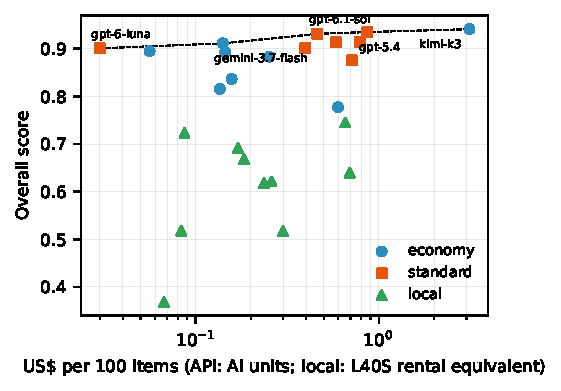
\includegraphics[width=\columnwidth]{pareto}
  \caption{Overall score against cost per 100 items (log scale; API: AI units at US\$0.01; local: GPU time at an on-demand L40S price). The dashed line joins the models that no other model beats at equal or lower cost.}
  \label{fig:pareto}
\end{figure}

The leaders are close in quality but not in price. Per 100 items, \TopName{} costs US\$\TopUSD{}, \SecondName{} US\$\SecondUSD{}, \ThirdName{} US\$\ThirdUSD{} and \FourthName{} US\$\FourthUSD{}. \CheapName{} reaches \CheapScore{}, \CheapGap{} below the leader, for US\$\CheapUSD{}, \CostRatio{} times less than \TopName{}. \ParetoN{} models form the cost--quality front (Fig.~\ref{fig:pareto}): \ParetoNames{}. Price does not follow the tiers we assigned by model names: \TopName{}, grouped with the economy models, is the most expensive per item because it reasons at length (median \TopMedS{}\,s per call against \ThirdMedS{}\,s for \ThirdName{}). The whole study cost US\$\StudyUSD{} in API calls---US\$\AnswerUSD{} for the answers, US\$\JudgeUSD{} for judging them and US\$\ProbeUSD{} for probing the premium models on two items each---and \GpuHours{} GPU-hours for the local models.

\subsection{What separates the models}
\label{sec:separates}
\input{generated/diagnostics\langsuffix}

Not the two knowledge-heavy tasks, which are near ceiling for API models: all \NApi{} answer at least \MethApiMin{} of the methodology questions correctly, and \LangCeil{} of them score at least 0.95 on formal Indonesian (the lowest \LangApiMin{}). This says that these items are too easy for API models, not that the models know the same. The tasks that produce artefacts separate them (Table~\ref{tab:diagnostics}).

\paragraph{References} The widest spread among API models is in the references task (\RefApiMin{}--\RefApiMax{}). Of the references the API models listed, \HalApiMin{}--\HalApiMax{}\,\% are not found in Crossref, and many found ones carry a wrong DOI: the share of listed references with the correct DOI ranges from \DoiApiMin{} to \DoiApiMax{}\,\%. The audit qualifies the misses. Of the \AuditApiNF{} references of API models that Crossref does not know, \AuditApiExact{}\,\% exist with matching title, year and first author in another source---works the Crossref-only score misses---, \AuditApiTitle{}\,\% match only the title of a real work (wrong year or author, or a coinciding generic title), and \AuditApiNone{}\,\% are found nowhere; for the \AuditLocNF{} misses of local models the shares are \AuditLocExact{}, \AuditLocTitle{} and \AuditLocNone{}\,\%. The audit's first pass exposed two Crossref pitfalls that the rule now handles (split subtitles, online-first dates). Per model, \NoneApiMin{}--\NoneApiMax{}\,\% of the references an API model listed are found nowhere (Fig.~\ref{fig:references}). Crediting the works the audit finds as the scorer would raises a references score by at most \VerRefMaxGain{} and leaves the ranking nearly unchanged (Spearman $\rho=\VerRho{}$, largest rank shift \VerMaxShift{}). Models also differ in caution: gpt-5-mini lists \RefsGptFiveMini{} references per item, \NoneGptFiveMini{}\,\% of them found nowhere, gemini-3.7-flash always lists five (\NoneGeminiThreeSevenFlash{}\,\%), and \TopName{} five (\NoneKimiKThree{}\,\%). Because the score counts abstention like an unverifiable reference, cautious models are not rewarded for listing fewer; the share found nowhere is the number to read for safety.

\begin{figure}[t]
  \centering
  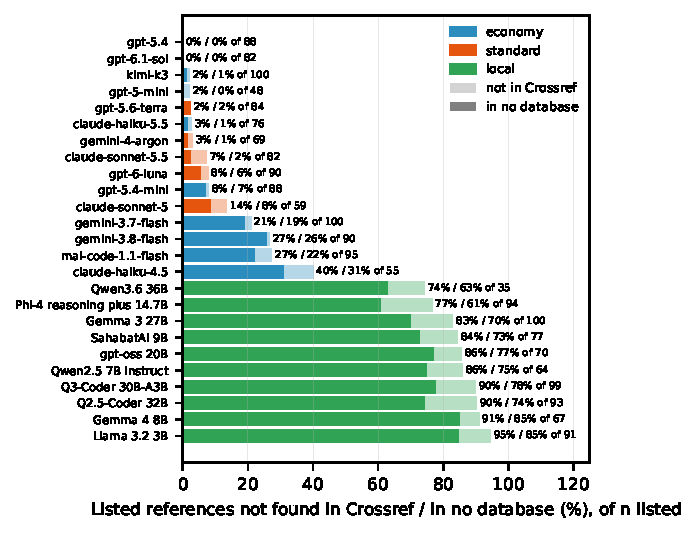
\includegraphics[width=\columnwidth]{references}
  \caption{Share of listed references not found in Crossref (light) and found in none of Crossref, doi.org, Scopus and OpenAlex (dark), with the number of references each model listed for the 20 topics (at most 100).}
  \label{fig:references}
\end{figure}

\paragraph{Outlines} Chapter outlines score \StructApiMin{}--\StructApiMax{} for API models. A frequent mismatch is the test-centred results chapter: \GenericApiMin{}--\GenericApiMax{}\,\% of the API outlines build chapter~IV around assumption, instrument or hypothesis tests for programmes whose theses do not organise their results that way.

\paragraph{Code and LaTeX} \ApiPerfectCode{} of the \NApi{} API models solve every coding task with their first program. Repairing a broken LaTeX document is harder than typesetting a table or a BibTeX entry, which all API models do correctly: the weakest API models produce a compilable document for only \FixApiMin{} of the broken ones.

\paragraph{Grounded writing} By the deterministic checks, API models keep to the given sources: at most \UnsupApiMax{} numbers per review occur in no source, and author--year citations, which the task forbids, appear in at most \ForeignApiMax{}\,\% of their reviews. Several local models ignore the citation format (author--year citations in up to \ForeignLocMax{}\,\% of their reviews).

\subsection{Local models}
\label{sec:local}
\begin{figure}[t]
  \centering
  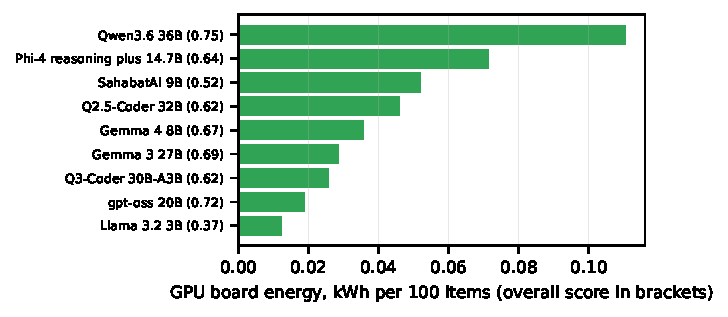
\includegraphics[width=\columnwidth]{energy}
  \caption{GPU board energy per 100 items of the local models (gross; shared server; Qwen2.5 7B not measured), with the overall score in brackets.}
  \label{fig:energy}
\end{figure}

The best local model, \BestLocalName{} (\BestLocalScore{}), stays below the weakest API model, \WorstApiName{} (\WorstApiScore{}). Between the group means the gap is largest for references (\GapRef{}) and code (\GapCode{}), smaller for methodology (\GapMeth{}) and smallest for formal Indonesian (\GapLang{}): local models write formal Indonesian at \LocLangMin{}--\LocLangMax{}, and Qwen3.6 36B scores \TMethodologyQwenThreeSix{} on the methodology questions. Of the references local models list, \NoneLocMin{}--\NoneLocMax{}\,\% are found nowhere, and they solve \LocPassOneMin{}--\LocPassOneMax{} of the coding tasks with their first program (mean \LocPassOneMean{}, rising to \LocRepairMean{} after one repair turn). The Indonesian-tuned SahabatAI 9B scores lower on formal Indonesian than the general Gemma~4 8B (\SahLang{} against \GemmaFourLang{}) and fails at code (\SahCode{}), so its overall score (\SahOverall{}) stays below Gemma~4's (\GemmaFourOverall{}). At an on-demand L40S price and three parallel requests, local models cost US\$\LocUSDMin{}--\LocUSDMax{} per 100 items, no less than the cheapest API models, and drew \LocKwhMin{}--\LocKwhMax{}\,kWh per 100 items (Fig.~\ref{fig:energy}); gpt-oss 20B gives the most score per kWh in this setup (\ScoreGptOss{} for \KwhGptOss{}\,kWh and US\$\UsdGptOss{} per 100 items).

\subsection{Judges and provenance}
The three judges rated \NJudgedAnswers{} answers with \NJudgeCalls{} ratings. On the \NAllJudges{} answers that all three rated (candidates from vendors other than the judges'), their mean ratings agree with Krippendorff's $\alpha=\AlphaJudges{}$ (interval); single criteria agree less ($\alpha$ from \AlphaCritMin{} to \AlphaCritMax{}, ordinal), least for instruction compliance and faithfulness. The judges' leniency differs by up to \LeniencyRange{} on the 0--1 scale, which the calibration removes. Their scores follow the deterministic checks: Spearman's $\rho$ is \RhoAnsGrd{} (grounded) and \RhoAnsLng{} (language) across answers, and \RhoModelGrd{} and \RhoModelLng{} across model means. The extraction panel agreed unanimously on \SilverUnanimous{}\,\% of the fields; analysis techniques were the hardest field (no majority on \SilverAnalysisNone{} of 30 excerpts, which are therefore not scored). In all \NApiCalls{} API calls of the study the SDK reported the requested model as the one that answered: the silent substitution reported for the same SDK when an account is not entitled to a model~\cite{arya2026paperagent} did not occur here. The check rests on the SDK's own usage event, not on an independent test of the backend.

\section{Discussion}
\label{sec:discussion}

\paragraph{Choosing a model} The leading API models are not significantly different on this benchmark, so price can decide among them: \ThirdName{} gives \ScoreGptSixOneSol{} for US\$\ThirdUSD{} per 100 items and gemini-3.7-flash \ScoreGeminiThreeSevenFlash{} for US\$\UsdGeminiThreeSevenFlash{}, against \TopScore{} for US\$\TopUSD{}; \CheapName{} (\CheapScore{} for US\$\CheapUSD{}) is the economical choice for high-volume use. The cheapest good models are not the ones with \emph{mini} or \emph{flash} in their names, and the most expensive model was not a flagship: measured cost per item is a better guide than tier labels.

\paragraph{References need a checker, whatever the model} \NoneApiNonzero{} of the \NApi{} API models listed references that no database knows, and many listed real works with a wrong DOI, year or author (Fig.~\ref{fig:references}). A reference produced by a model should be verified before it enters a thesis; a lookup in Crossref, with a second database for the misses, costs next to nothing compared with a fabricated citation in an examined document. Thesis tools should treat references as a retrieval problem, not a generation problem.

\paragraph{Local models} Local models are the option when data may not leave the institution, and for the tasks where they come close to API models: rewriting text into formal Indonesian and answering methodology questions. They were not cheaper per item at rental prices than the cheapest API models of much higher quality, and they should not be trusted with references. The model tuned for Indonesian did not outperform a newer general model of its size, which suggests that for these tasks a recent general model is a better starting point than language specialisation alone (one pair of models with different quantisation; not a controlled comparison).

\paragraph{Benchmark design} Two tasks are near ceiling for API models (methodology, formal Indonesian) while still separating local models; harder variants---open questions, longer drafts with subtler non-standard forms---would extend their range. Judging was the largest cost item. Scoring the prose tasks by the deterministic checks alone barely changes the overall ranking (Spearman $\rho=\JudgeAutoRho{}$, largest rank shift \JudgeAutoShift{}), so judging a stratified sample of answers may suffice; we have not tested this.

\paragraph{Limitations} Each model answered each item once, at low reasoning effort, so run-to-run variation is not measured; the \NPremium{} premium-tier models (estimated at about US\$50) and a high-effort check of the best models are not in this version. AI units are the vendor's billing measure at one point in time, hosted models change without notice, and the served-model check relies on the SDK's report. The structure references and the extraction excerpts come from the theses of one university; extraction is scored against silver labels, which for a candidate come from the panel members of other vendors and therefore differ between vendors; the extraction items are private, but without them the ranking is almost the same (Spearman $\rho=\PubRho{}$, largest rank shift \PubMaxShift{}). Neither the LLM judges nor the item keys have yet been checked by people, and the items were drafted with LLM assistance, which may favour LLM phrasing; deterministic scoring limits this risk but does not remove it. The grounded checks test citation form, coverage and numbers, not whether each cited claim is supported, which is left to the judges. A real work that none of the four databases knows counts as not found. Local models ran 4-bit quantised in one serving stack, their energy was measured on a shared server, and their cost depends on the concurrency used.

\section{Conclusion}
\label{sec:conclusion}

AcademicBench measures several things that Indonesian thesis work needs from an LLM---outlines that fit the study programme, faithful use of sources, real references, formal Indonesian, correct analysis code and compilable LaTeX---together with what each answer costs and which model produced it. Across \NModels{} models, the three best API models are not significantly different while the cost of the API models spans two orders of magnitude, references separate the models most, and on average local models trail on every task, least on formal Indonesian. The practical advice is to choose by price among the leaders, to verify every reference, and to use local models where privacy requires it. The kit evaluates any further model with one command; the premium tier, high reasoning effort, repeated runs and a human check of the judges and keys are the next steps.


\bibliographystyle{IEEEtran}
\bibliography{references}

\end{document}
